\section{Date: 2026-10-13}
\noindent \textbf{Series ID: APUB30074714} 

\noindent This series is titled Average Price: Gasoline, Unleaded Regular (Cost per Gallon/3.785 Liters) in the South Census Region - Size Class B and has a frequency of Monthly. The units are U.S. Dollars and the seasonal adjustment is Not Seasonally Adjusted.The observation start date is 1978-01-01 and the observation end date is 1997-12-01.The popularity of this series is 1. \\ 

\noindent \textbf{Series ID: FHA30} 

\noindent This series is titled 30-Year FHA Mortgage Rate: Secondary Market (DISCONTINUED) and has a frequency of Monthly. The units are Percent and the seasonal adjustment is Not Seasonally Adjusted.The observation start date is 1964-01-01 and the observation end date is 2000-06-01.The popularity of this series is 9. \\ 

\subsection{Raw Regression}
\noindent Regresses the two series against each other directly. A significant result here can come just as easily from both series sharing a long-run trend as from any real relationship.

\begin{center}
\begin{tabular}{lclc}
\toprule
\textbf{Dep. Variable:}            & value\_fred\_FHA30 & \textbf{  R-squared:         } &     0.169   \\
\textbf{Model:}                    &        OLS         & \textbf{  Adj. R-squared:    } &     0.165   \\
\textbf{Method:}                   &   Least Squares    & \textbf{  F-statistic:       } &     47.29   \\
\textbf{Date:}                     &  Tue, 13 Oct 2026  & \textbf{  Prob (F-statistic):} &  5.59e-11   \\
\textbf{Time:}                     &      18:35:32      & \textbf{  Log-Likelihood:    } &   -534.79   \\
\textbf{No. Observations:}         &          235       & \textbf{  AIC:               } &     1074.   \\
\textbf{Df Residuals:}             &          233       & \textbf{  BIC:               } &     1081.   \\
\textbf{Df Model:}                 &            1       & \textbf{                     } &             \\
\textbf{Covariance Type:}          &     nonrobust      & \textbf{                     } &             \\
\bottomrule
\end{tabular}
\begin{tabular}{lcccccc}
                                   & \textbf{coef} & \textbf{std err} & \textbf{t} & \textbf{P$> |$t$|$} & \textbf{[0.025} & \textbf{0.975]}  \\
\midrule
\textbf{const}                     &       3.5713  &        1.048     &     3.408  &         0.001        &        1.507    &        5.636     \\
\textbf{value\_fred\_APUB30074714} &       6.5135  &        0.947     &     6.876  &         0.000        &        4.647    &        8.380     \\
\bottomrule
\end{tabular}
\begin{tabular}{lclc}
\textbf{Omnibus:}       & 11.293 & \textbf{  Durbin-Watson:     } &    0.039  \\
\textbf{Prob(Omnibus):} &  0.004 & \textbf{  Jarque-Bera (JB):  } &    6.092  \\
\textbf{Skew:}          &  0.195 & \textbf{  Prob(JB):          } &   0.0476  \\
\textbf{Kurtosis:}      &  2.315 & \textbf{  Cond. No.          } &     13.6  \\
\bottomrule
\end{tabular}
%\caption{OLS Regression Results}
\end{center}

Notes: \newline
 [1] Standard Errors assume that the covariance matrix of the errors is correctly specified.

\begin{figure}
\centering
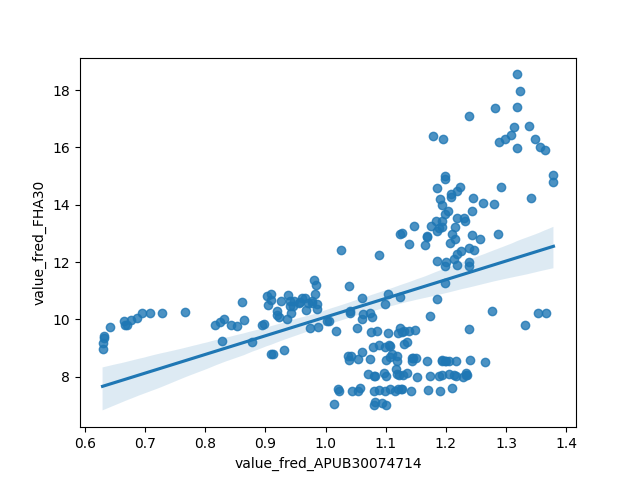
\includegraphics[scale = 0.9]{plots/plot_2026-10-13.png}
\caption{Raw Regression Plot for 2026-10-13}
\end{figure}
\newpage
\subsection{Detrended Regression}
\noindent Regresses the residuals of each series after removing its own linear time trend, so a shared trend can no longer drive the result on its own. A relationship that stays significant here is better evidence of a genuine link between the two series.

\begin{center}
\begin{tabular}{lclc}
\toprule
\textbf{Dep. Variable:}                       & value\_fred\_FHA30\_detrended & \textbf{  R-squared:         } &     0.626   \\
\textbf{Model:}                               &              OLS              & \textbf{  Adj. R-squared:    } &     0.624   \\
\textbf{Method:}                              &         Least Squares         & \textbf{  F-statistic:       } &     389.6   \\
\textbf{Date:}                                &        Tue, 13 Oct 2026       & \textbf{  Prob (F-statistic):} &  1.23e-51   \\
\textbf{Time:}                                &            18:35:32           & \textbf{  Log-Likelihood:    } &   -352.60   \\
\textbf{No. Observations:}                    &                235            & \textbf{  AIC:               } &     709.2   \\
\textbf{Df Residuals:}                        &                233            & \textbf{  BIC:               } &     716.1   \\
\textbf{Df Model:}                            &                  1            & \textbf{                     } &             \\
\textbf{Covariance Type:}                     &           nonrobust           & \textbf{                     } &             \\
\bottomrule
\end{tabular}
\begin{tabular}{lcccccc}
                                              & \textbf{coef} & \textbf{std err} & \textbf{t} & \textbf{P$> |$t$|$} & \textbf{[0.025} & \textbf{0.975]}  \\
\midrule
\textbf{const}                                &    5.561e-13  &        0.071     &  7.82e-12  &         1.000        &       -0.140    &        0.140     \\
\textbf{value\_fred\_APUB30074714\_detrended} &       8.7393  &        0.443     &    19.738  &         0.000        &        7.867    &        9.612     \\
\bottomrule
\end{tabular}
\begin{tabular}{lclc}
\textbf{Omnibus:}       &  5.577 & \textbf{  Durbin-Watson:     } &    0.209  \\
\textbf{Prob(Omnibus):} &  0.062 & \textbf{  Jarque-Bera (JB):  } &    5.236  \\
\textbf{Skew:}          &  0.334 & \textbf{  Prob(JB):          } &   0.0729  \\
\textbf{Kurtosis:}      &  3.299 & \textbf{  Cond. No.          } &     6.23  \\
\bottomrule
\end{tabular}
%\caption{OLS Regression Results}
\end{center}

Notes: \newline
 [1] Standard Errors assume that the covariance matrix of the errors is correctly specified.

\begin{figure}
\centering
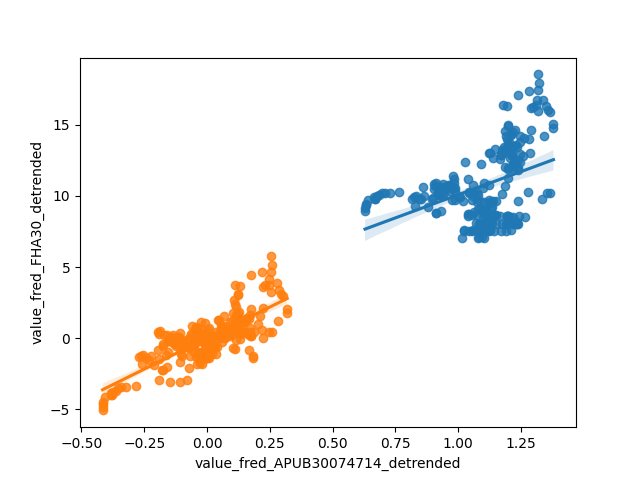
\includegraphics[scale = 0.9]{plots/plot_2026-10-13_detrended.png}
\caption{Detrended Regression Plot for 2026-10-13}
\end{figure}
\newpage
